\documentclass[12pt, a4paper]{article}

\usepackage{listings}
\usepackage{graphicx}
\usepackage{hyperref}
\usepackage{float}

%opening
\title{Data Mining: Frequent Itemsets and Association rules}
\author{Braulio Grana Guti\'errez \and Adri\'an Ram\'irez del R\'io}

\begin{document}

\maketitle

\section{Description}

\subsection{Algorithm}
For this assignment we had to implement the Spectral Clustering algorithm \cite{speclust01}. To do so, we used MATLAB and the \emph{Statistics and Machine Learning Toolbox}.

We created a function that receives a list of edges \emph{E} and the number \emph{k} as parameters, and implemented the algorithm with the following steps:

\begin{enumerate}
\item We use the adjacency matrix \emph{A} as affinity matrix.
\item Build the degree matrix \emph{D}, which is a diagonal matrix whose \emph{(i,i)-elements} are the sum of A's \emph{i-th} row.
\item Build the normalized Laplacian matrix \emph{L} using the following formula:
\begin{center}
$L = D^{1/2} \times A \times D^{1/2}$
\end{center}
\item Build matrix \emph{X} by finding the k largest eigenvectors of L and stacking them in columns. For this we used the MATLAB method \emph{eigs}.
\item Renormalize each row of \emph{X} to have unit length (Store the result in \emph{Y})
\item Use K-means from the \emph{Statistics and Machine Learning Toolbox} to find the \emph{k} clusters in \emph{Y}.
\item Assign each original point to its cluster and return the result \emph{C}.

\end{enumerate}

Our function returns a vector \emph{C} with tuples containing a point and its assigned cluster. 

\subsection{Example datasets analysis}

When analysing the examples, we used the sparsity pattern plot to see the number of possible patterns and decide the \emph{k} parameter.

\subsubsection{Example 1}
For the first example, which is a real world graph based in the medical data collection from 4 towns, we have the following sparsity pattern:

\begin{figure}[H]
\centering
	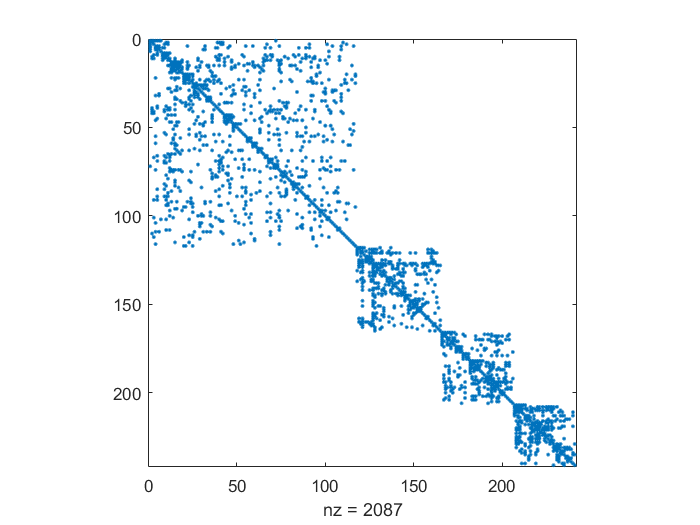
\includegraphics[width=0.8\textwidth]{../plots/sparsity_ex1.png}
	\caption{Sparsity pattern for example 1}
\end{figure}

From this pattern we can easily see that we probably have 4 clusters, so we tried the algorithm with \emph{k = 4} and this is the result when showing the clusters over fiedler vector:

\begin{figure}[H]
\centering
	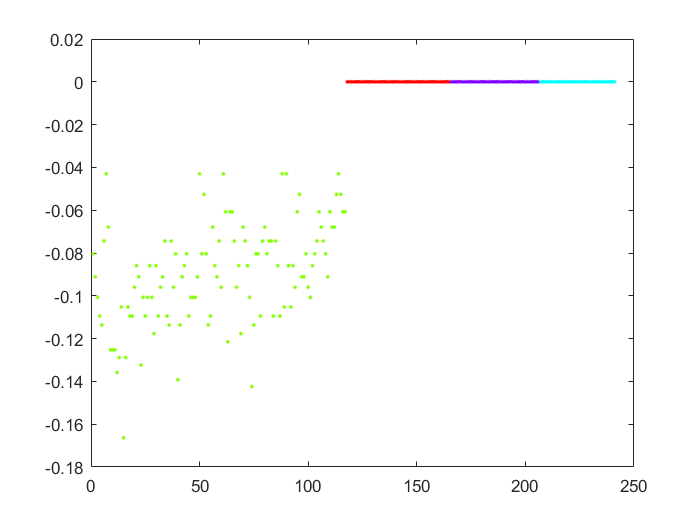
\includegraphics[width=0.6\textwidth]{../plots/clusters_ex1.png}
	\caption{Clusters over fiedler vector for example 1}
\end{figure}

\subsubsection{Example 2}
For the second example, which is a generated graph, we found no clusters in the sparsity pattern plot as can be seen in \autoref{fig:sparsity2}:

\begin{figure}[H]
\centering
	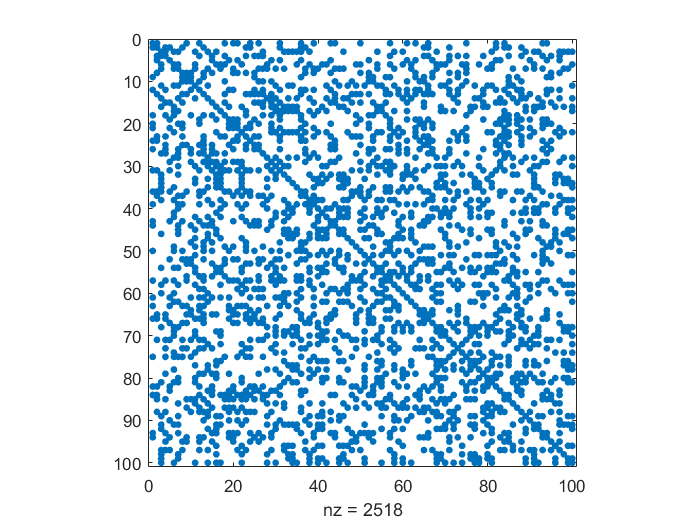
\includegraphics[width=0.8\textwidth]{../plots/sparsity_ex2.png}
	\caption{Sparsity pattern for example 2}
	\label{fig:sparsity2}
\end{figure}

Therefore, we tried several values of \emph{k} until we found one (\emph{k = 2}) that showed a reasonable clustering over the fiedler vector:

\begin{figure}[H]
\centering
	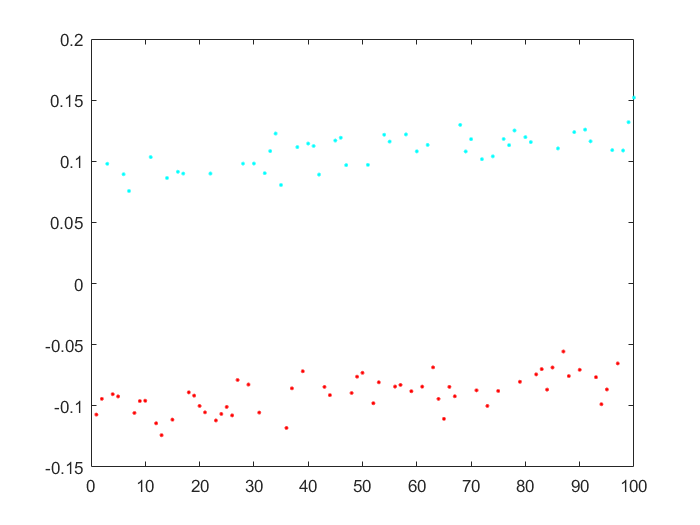
\includegraphics[width=0.6\textwidth]{../plots/clusters_ex2.png}
	\caption{Clusters over fiedler vector for example 2}
\end{figure}

\section{Instructions}
To use our implementation:
\begin{enumerate}
\item Open MATLAB and change the current folder to the project root.
\item Then, in the MATLAB console, execute the following commands:
\lstset{language=MATLAB}
\begin{lstlisting}[frame=single]
E = readcsv('Path_to_dataset');
C = SpectralClustering(E, k);
\end{lstlisting}
\end{enumerate}

\begin{thebibliography}{2}

\bibitem{speclust01}
  Andrew Ng, Michael I. Jordan and Yar Weiss,
  \emph{On Spectral Clustering: Analysis and algorithm},
  2001.

\bibitem{luxburg07}
  Ulrike von Luxburg,
  \emph{A tutorial on Spectral Clustering},
  2007.

\end{thebibliography}


\end{document}